\section{Exercise 4}

\newcommand{\foldnode}[2]{
    \node[minimum height=0.7cm, minimum width=0.4cm, fill=#2, draw=black] at #1 {};
}

\begin{frame}{Exercise 4: Data splitting}
    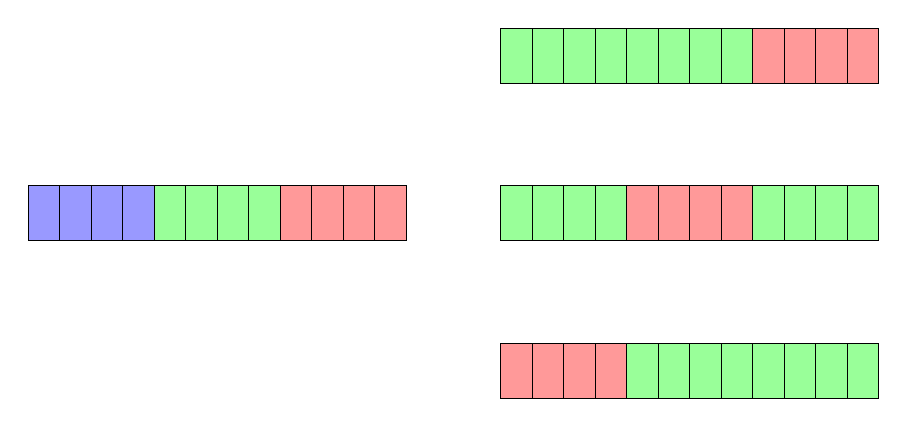
\begin{tikzpicture}
        \visible<1-2>{
            \foldnode{(0, 0)}{blue!40};
            \foldnode{(0.4, 0)}{blue!40};
            \foldnode{(0.8, 0)}{blue!40};
            \foldnode{(1.2, 0)}{blue!40};
            \foldnode{(1.6, 0)}{blue!40};
            \foldnode{(2.0, 0)}{blue!40};
            \foldnode{(2.4, 0)}{blue!40};
            \foldnode{(2.8, 0)}{blue!40};
            \foldnode{(3.2, 0)}{blue!40};
            \foldnode{(3.6, 0)}{blue!40};
            \foldnode{(4, 0)}{blue!40};
            \foldnode{(4.4, 0)}{blue!40};
        }
        \visible<2>{
            \foldnode{(6, 2)}{green!40};
            \foldnode{(6.4, 2)}{green!40};
            \foldnode{(6.8, 2)}{green!40};
            \foldnode{(7.2, 2)}{green!40};
            \foldnode{(7.6, 2)}{green!40};
            \foldnode{(8.0, 2)}{green!40};
            \foldnode{(8.4, 2)}{green!40};
            \foldnode{(8.8, 2)}{green!40};
            \foldnode{(9.2, 2)}{red!40};
            \foldnode{(9.6, 2)}{red!40};
            \foldnode{(10, 2)}{red!40};
            \foldnode{(10.4, 2)}{red!40};

            \foldnode{(6, 0)}{green!40};
            \foldnode{(6.4, 0)}{green!40};
            \foldnode{(6.8, 0)}{green!40};
            \foldnode{(7.2, 0)}{green!40};
            \foldnode{(7.6, 0)}{red!40};
            \foldnode{(8.0, 0)}{red!40};
            \foldnode{(8.4, 0)}{red!40};
            \foldnode{(8.8, 0)}{red!40};
            \foldnode{(9.2, 0)}{green!40};
            \foldnode{(9.6, 0)}{green!40};
            \foldnode{(10, 0)}{green!40};
            \foldnode{(10.4, 0)}{green!40};

            \foldnode{(6, -2)}{red!40};
            \foldnode{(6.4, -2)}{red!40};
            \foldnode{(6.8, -2)}{red!40};
            \foldnode{(7.2, -2)}{red!40};
            \foldnode{(7.6, -2)}{green!40};
            \foldnode{(8.0, -2)}{green!40};
            \foldnode{(8.4, -2)}{green!40};
            \foldnode{(8.8, -2)}{green!40};
            \foldnode{(9.2, -2)}{green!40};
            \foldnode{(9.6, -2)}{green!40};
            \foldnode{(10, -2)}{green!40};
            \foldnode{(10.4, -2)}{green!40};
        }
        \visible<3>{
            \foldnode{(0, 0)}{blue!40};
            \foldnode{(0.4, 0)}{blue!40};
            \foldnode{(0.8, 0)}{blue!40};
            \foldnode{(1.2, 0)}{blue!40};
            \foldnode{(1.6, 0)}{green!40};
            \foldnode{(2.0, 0)}{green!40};
            \foldnode{(2.4, 0)}{green!40};
            \foldnode{(2.8, 0)}{green!40};
            \foldnode{(3.2, 0)}{red!40};
            \foldnode{(3.6, 0)}{red!40};
            \foldnode{(4, 0)}{red!40};
            \foldnode{(4.4, 0)}{red!40};
        }
    \end{tikzpicture}
\end{frame}
